\begin{figure}
    \caption{Decisi\'on de tema de proyecto final\label{fig:No.1}}
    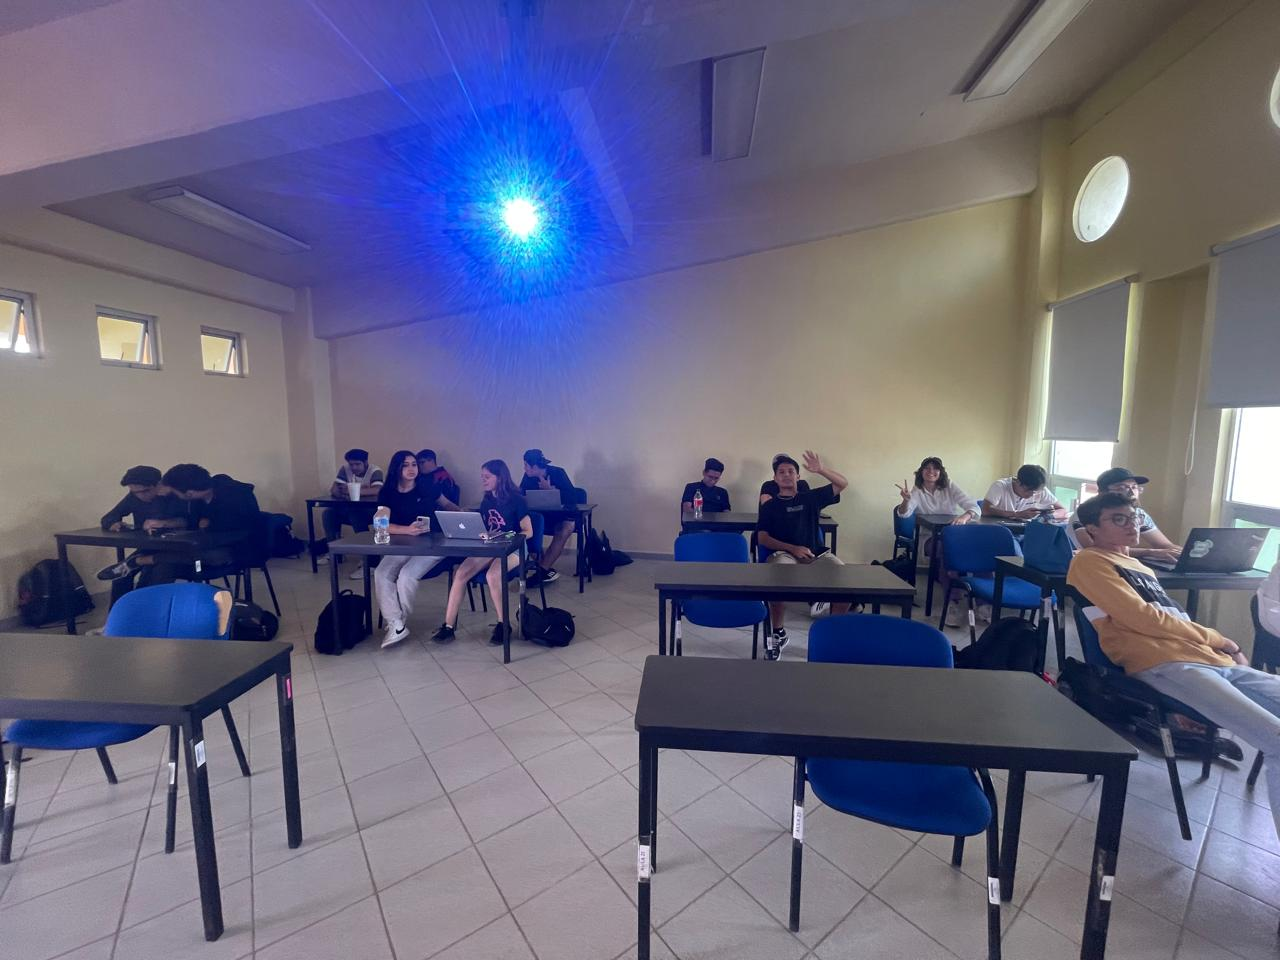
\includegraphics[width=0.7\textwidth]{./assets/img/imagen2DH.jpeg}
	\textit{Nota.} Fecha de la fotograf\'ia: El d\'ia 10 de marzo del 2024 se llev\'o a cabo la decisi\'on sobre el tema del proyecto final y se asignaron los respectivos roles. Grupo 31, 2024.
\end{figure}

\begin{figure}
    \caption{Retroalimentaci\'on.\label{fig:No.2}}
    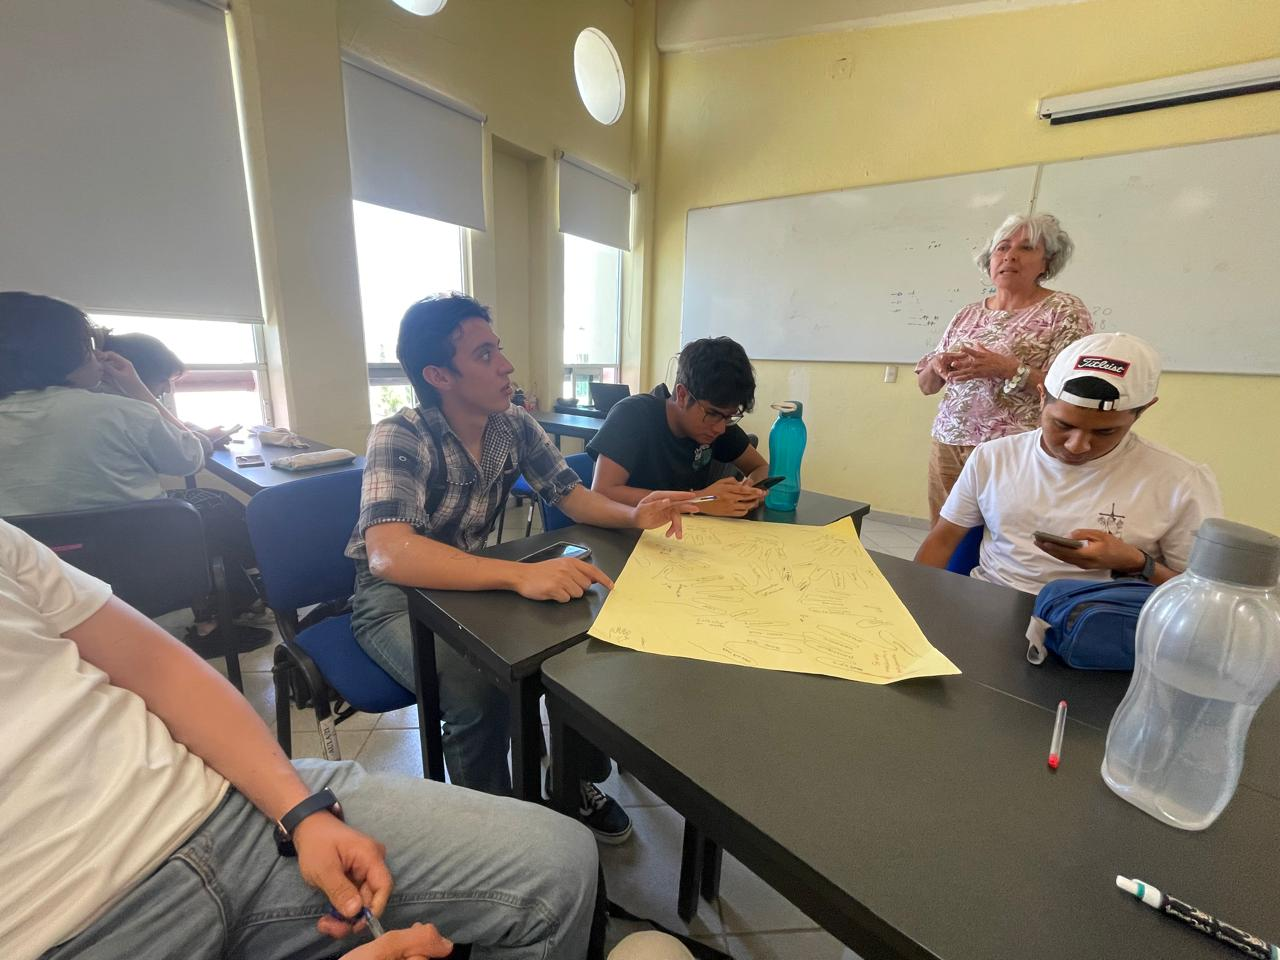
\includegraphics[width=0.7\textwidth]{./assets/img/imagen1DH.jpeg}
	\textit{Nota.} El d\'ia 21 de marzo del 2024 se realiz\'o una actividad de retroalimentaci\'on sobre el tema ``Inteligencias M\'ultiples''
\end{figure}

\begin{figure}
    \caption{Clase de inteligencia emocional\label{fig:No.3}}
    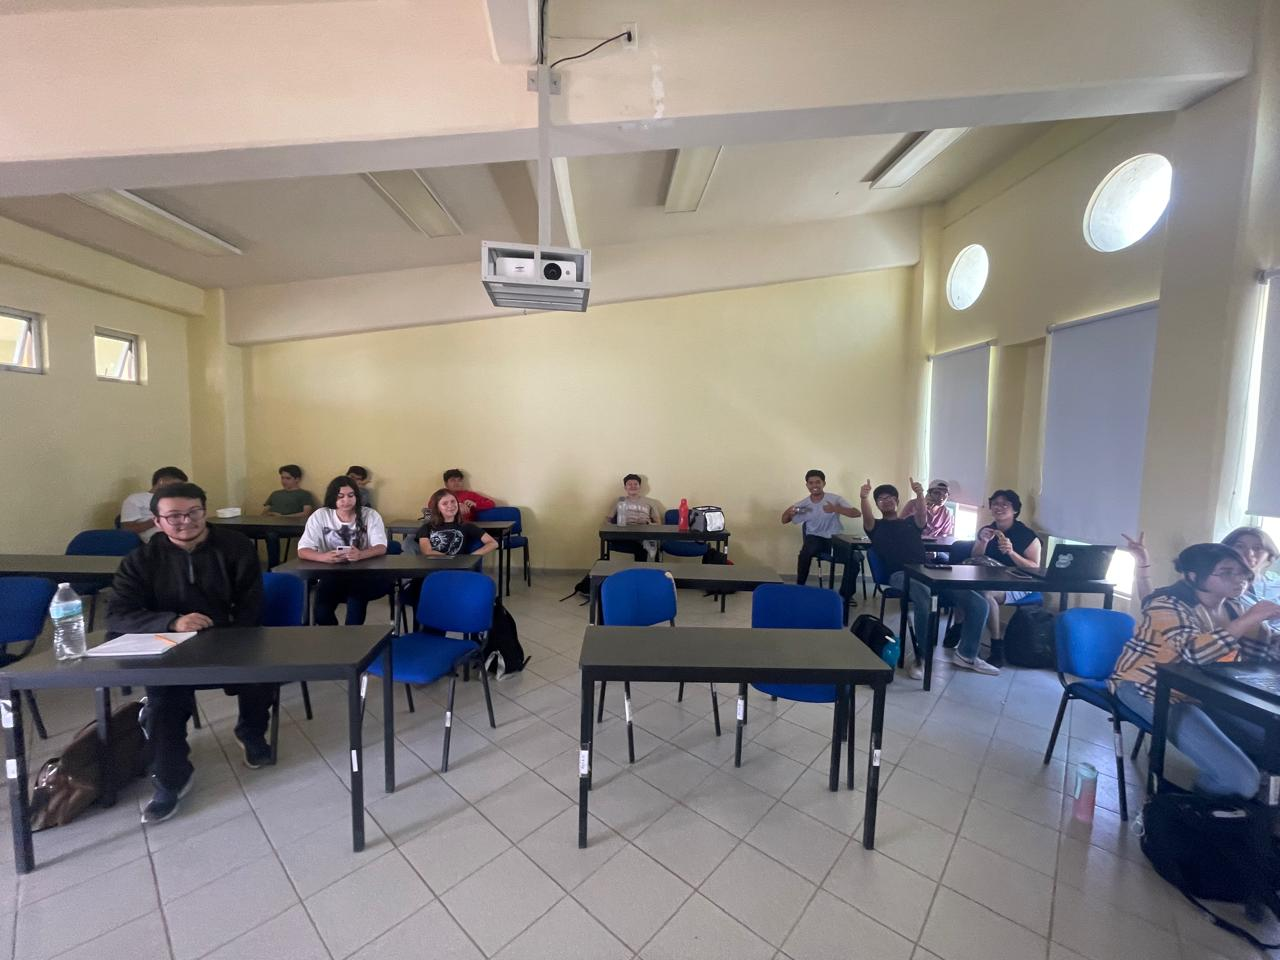
\includegraphics[width=0.7\textwidth]{./assets/img/imagen3DH.jpeg}
	\textit{Nota.} El d\'ia 2 de Mayo de 2024 se llev\'o a cabo la clase enfocada a la inteligencia emocional en el ámbito laboral. Grupo 31, 2024.
\end{figure}

\begin{figure}
    \caption{Hincapi\'e en la r\'ubrica de evaluaci\'on\label{fig:No.4}}
    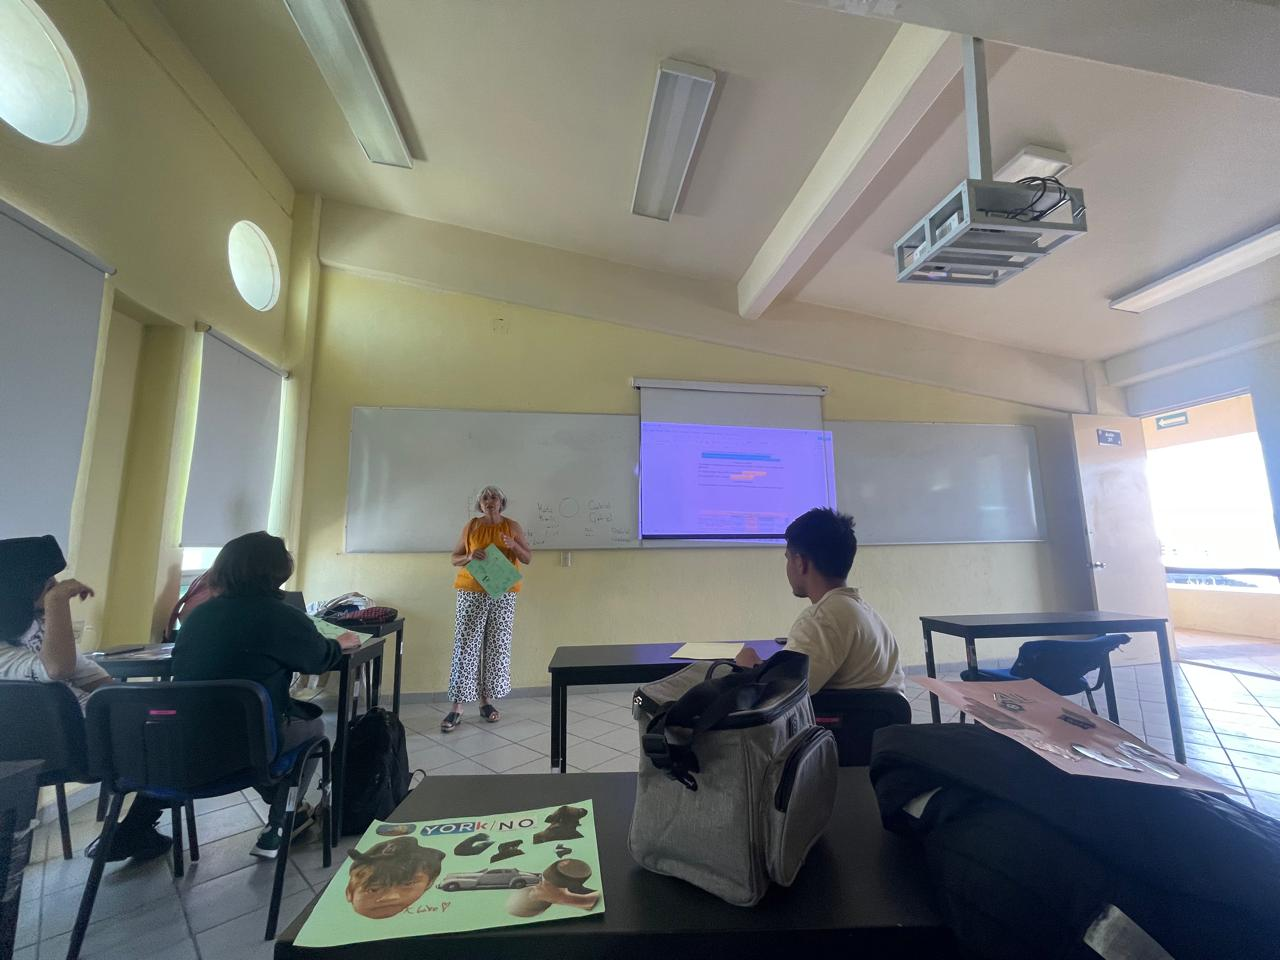
\includegraphics[width=0.7\textwidth]{./assets/img/imagen4DH.jpeg}
	\textit{Nota.} El día 7 de mayo de 2024 se hizo incapi\'e en la r\'ubrica de evaluaci\'on del proyecto final de la materia ``Desarrollo Humano II''. Grupo 31, 2024.
\end{figure}

\begin{figure}
    \caption{Actividad din\'amica\label{fig:No.5}}
    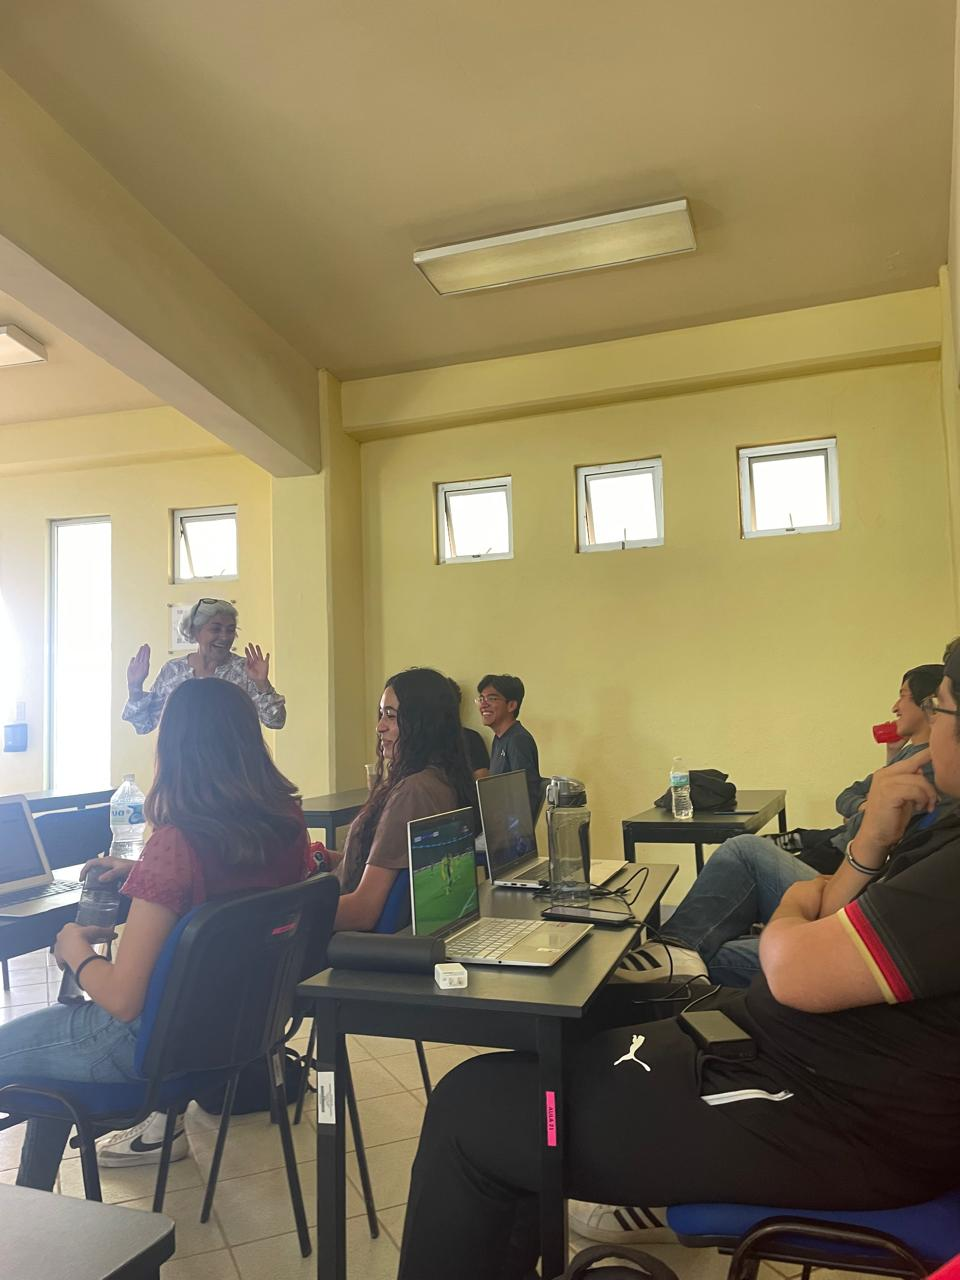
\includegraphics[width=0.7\textwidth]{./assets/img/imagen5DH.jpeg}
	\textit{Nota.} El d\'ia 14 de mayo de 2024 se realiz\'o una actividad recreativa haciendo uso de la m\'imica con la inteligencia visual-espacial. Grupo 31,2024.
\end{figure}

\begin{figure}
    \caption{Evaluaci\'on tercer parcial\label{fig:No.6}}
    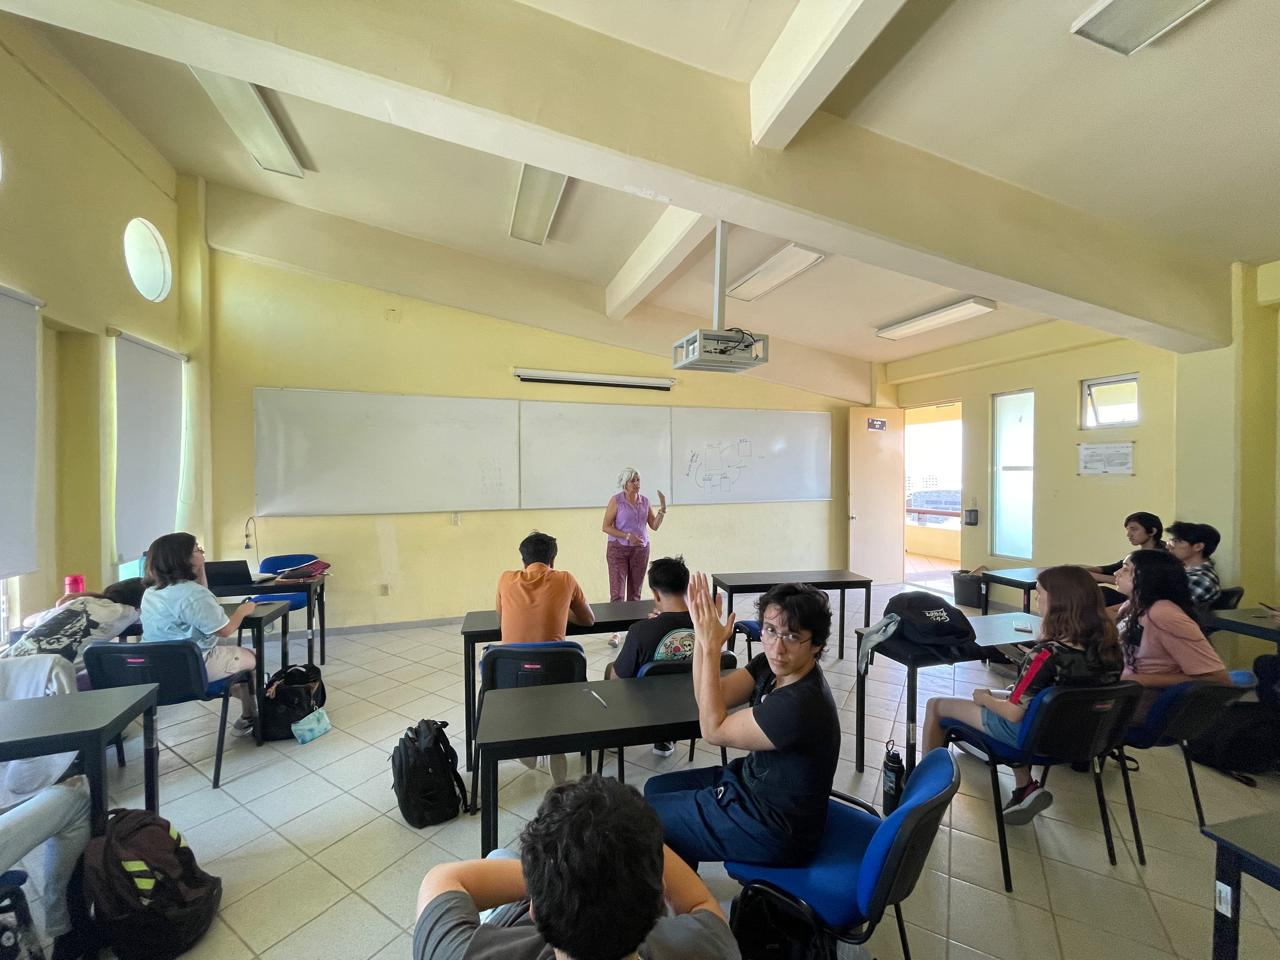
\includegraphics[width=0.7\textwidth]{./assets/img/imagen6DH.jpeg}
	\textit{Nota.} El d\'ia 16 de mayo de 2024 se llev\'o a cabo el examen del 3er Parcial de la materia ``Desarrollo Humano II''. Grupo 31, 2024.
\end{figure}
